\chapter{Acoustic Solver}

\section{Synopsis}
The aim of the AcousticSolver is to predict acoustic wave propagation.
Through the application of a splitting technique, the flow-induced acoustic field is
totally decoupled from the underlying hydrodynamic field.

\subsection{Linearized Euler Equations}
The Linearized Euler Equations (LEE) are obtained by linearizing the Euler Equations about a mean flow state $\left( \overline{\rho},\,\overline{c^2},\,\overline{\boldsymbol{u}} \right)$.
Hence, they describe the evolution of perturbations $\left(p^\mathrm{a},\,\rho^\mathrm{a},\,\overline{\rho}\boldsymbol{u}^\mathrm{a} \right)$ around this state.
In conservative form, the LEE are given as:
\begin{equation} 
\frac{\partial \boldsymbol{U}}{\partial t}
+ \frac{\partial \boldsymbol{F}_1}{\partial x_1}
+ \frac{\partial \boldsymbol{F}_2}{\partial x_2}
+ \frac{\partial \boldsymbol{F}_3}{\partial x_3}
    + \boldsymbol{C}   \boldsymbol{U}
= \boldsymbol{W}
\end{equation}
with
\begin{gather}
\boldsymbol{U} =  \left[\begin{matrix}
    p^\mathrm{a}\\ 
    \rho^a\\
    \overline{\rho}u^a_1\\ 
    \overline{\rho}u^a_2\\
    \overline{\rho}u^a_3
\end{matrix}\right],
\\ 
\boldsymbol{F}_1 = \left[\begin{matrix}
    \overline{\rho}u^a_1 \overline{c^2} + \overline{u}_1 p^\mathrm{a}\\
    \overline{\rho}u^a_1 + \overline{u}_1 \rho^a\\
    \overline{\rho}u^a_1 \overline{u}_1 + p^\mathrm{a}\\
    \overline{\rho}u^a_2 \overline{u}_1\\
    \overline{\rho}u^a_3 \overline{u}_1
\end{matrix}\right],
\quad 
\boldsymbol{F}_2 = \left[\begin{matrix}
    \overline{\rho}u^a_2 \overline{c^2} + \overline{u}_2 p^\mathrm{a}\\
    \overline{\rho}u^a_2 + \overline{u}_2 \rho^a\\
    \overline{\rho}u^a_1 \overline{u}_2\\
    \overline{\rho}u^a_2 \overline{u}_2 + p^\mathrm{a}\\
    \overline{\rho}u^a_3 \overline{u}_2
\end{matrix}\right],
\quad 
\boldsymbol{F}_3 = \left[\begin{matrix}
    \overline{\rho}u^a_3 \overline{c^2} + \overline{u}_3 p^\mathrm{a}\\
    \overline{\rho}u^a_3 + \overline{u}_3 \rho^a\\
    \overline{\rho}u^a_1 \overline{u}_3\\
    \overline{\rho}u^a_2 \overline{u}_3\\
    \overline{\rho}u^a_3 \overline{u}_3 + p^\mathrm{a}
\end{matrix}\right], 
\\
\boldsymbol{C} = \left[\begin{matrix}
    \left(\gamma - 1\right) \frac{\partial \overline{u}_k}{\partial x_k}  & 0 & \frac{1}{\overline{\rho}} \left(1 - \gamma\right) \frac{\partial \overline{p}}{\partial x_1} & \frac{1}{\overline{\rho}} \left(1 - \gamma\right) \frac{\partial \overline{p}}{\partial x_2} & \frac{1}{\overline{\rho}} \left(1 - \gamma\right) \frac{\partial \overline{p}}{\partial x_3} \\
    0 & 0 & 0 & 0 & 0\\
    0 & \overline{u}_k \frac{\partial \overline{u}_1 }{\partial x_k} & \frac{\partial \overline{u}_1}{\partial x_1}  & \frac{\partial \overline{u}_1}{\partial x_2}  & \frac{\partial \overline{u}_1}{\partial x_3} \\
    0 & \overline{u}_k \frac{\partial \overline{u}_2}{\partial x_k}  & \frac{\partial \overline{u}_2}{\partial x_1}  & \frac{\partial \overline{u}_2}{\partial x_2}  & \frac{\partial \overline{u}_2}{\partial x_3} \\
    0 & \overline{u}_k \frac{\partial  \overline{u}_3}{\partial x_k} & \frac{\partial \overline{u}_3}{\partial x_1}  & \frac{\partial \overline{u}_3}{\partial x_2}  & \frac{\partial \overline{u}_3}{\partial x_3} 
\end{matrix}\right]
\;.
\end{gather}
By default, the source term vector $\boldsymbol{W}$ is zero and has to be specified by an appropriate forcing.


\subsection{Acoustic Perturbation Equations}
The acoustic perturbation equations (APE-1/APE-4) proposed by Ewert and Schroeder \cite{EwSc03} assure stable aeroacoustic simulations.
These equations are similar to the LEE, but account for acoustic perturbations exclusively.
The AcousticSolver implements the APE-1/4 type operator:
\begin{subequations}
    \begin{align}
        \frac{\partial p^{\mathrm{a}}}{\partial t} 
        + \overline{c^2} \nabla \cdot \left( \overline{\rho}
        \boldsymbol{u}^{\mathrm{a}} 
        + \overline{\boldsymbol{u}} \frac{p^{\mathrm{a}}}{\overline{c^2}} \right) 
        &= \dot{\omega}_{\mathrm{c}}
        \\
        \frac{\partial \boldsymbol{u}^{\mathrm{a}}}{\partial t} 
        + \nabla \left(\overline{\boldsymbol{u}} \cdot
        \boldsymbol{u}^{\mathrm{a}} \right) 
        + \nabla \left(\frac{p^{\mathrm{a}}}{\overline{\rho}}\right) 
        &= \dot{\boldsymbol{\omega}}_{\mathrm{m}}
        \;,
    \end{align}
\end{subequations}
where $(\overline{\boldsymbol{u}},\,\overline{c^2},\, \overline{\rho})$
represents the base flow and $(\boldsymbol{u}^{\mathrm{a}},p^{\mathrm{a}})$ the acoustic perturbations.
Similar to the LEE, the acoustic source terms $\dot{\omega}_{\mathrm{c}}$ and
$\dot{\boldsymbol{\omega}}_{\mathrm{m}}$ are by default zero and must be specified e.g. by an appropriate forcing.
This way, e.g. the APE-1, APE-4 \cite{EwSc03} or revised APE equations \cite{Ge14} can be obtained.
Expressed as hyperbolic conservation law, the APE-1/4 operator reads:
\begin{equation}
\frac{\partial  \boldsymbol{U}}{\partial t}
+ \frac{\partial \boldsymbol{F}_1}{\partial x_1}
+ \frac{\partial \boldsymbol{F}_2}{\partial x_2}
+ \frac{\partial \boldsymbol{F}_3}{\partial x_3}
= \boldsymbol{W}
\end{equation}
with
\begin{gather}
\boldsymbol{U} = \left[
\begin{matrix}
    p^{\mathrm{a}} \\
    u^{\mathrm{a}}_1 \\
    u^{\mathrm{a}}_2 \\
    u^{\mathrm{a}}_3
\end{matrix}
\right] , \\
\boldsymbol{F_1} = \left[
\begin{matrix}
    \overline{\rho} \overline{c^2} u^{\mathrm{a}}_1 + p^{\mathrm{a}} \overline{u}_1  \\
    \overline{u}_j u^{\mathrm{a}}_j + p^{\mathrm{a}} / \overline{\rho}  \\
0 \\
0
\end{matrix}
\right]     , \;
\boldsymbol{F_2} = \left[
\begin{matrix}
    \overline{\rho} \overline{c^2} u^{\mathrm{a}}_2 + p^{\mathrm{a}} \overline{u}_2  \\
0 \\
    \overline{u}_j u^{\mathrm{a}}_j + p^{\mathrm{a}} / \overline{\rho}  \\
0
\end{matrix}
\right]    , \;
\boldsymbol{F_3} = \left[
\begin{matrix}
    \overline{\rho} \overline{c^2} u^{\mathrm{a}}_3 + p^{\mathrm{a}} \overline{u}_3 \\
0     \\
0     \\
    \overline{u}_j u^{\mathrm{a}}_j + p^{\mathrm{a}} / \overline{\rho}  \\
\end{matrix}
\right]
\,.
\end{gather}







\section{Usage}
\begin{lstlisting}[style=BashInputStyle]
AcousticSolver session.xml
\end{lstlisting}

\section{Session file configuration}

\subsection*{Parameters}
Under this section it is possible to set the parameters of the simulation.
\begin{lstlisting}[style=XmlStyle]
<PARAMETERS>
  <P> TimeStep       = 1e-05  /P>
  <P> NumSteps       = 1000   /P>
  <P> FinTime        = 0.01   /P>
  <P> IO_CheckSteps  = 100    /P>
  <P> IO_InfoSteps   = 10     /P>
  <P> IO_CFLSteps    = 10     /P>
</PARAMETERS>
\end{lstlisting}
\begin{itemize}
    \item \inltt{TimeStep} is the time-step we want to use;
    \item \inltt{FinTime} is the final physical time at which we want our simulation to stop;
    \item \inltt{NumSteps} is the equivalent of \inltt{FinTime} but instead of specifying the physical final time we specify the number of time-steps;
    \item \inltt{IO\_CheckSteps} sets the number of steps between successive checkpoint files;
    \item \inltt{IO\_InfoSteps} sets the number of steps between successive info stats are printed to screen;
    \item \inltt{IO\_CFLSteps} sets the number of steps between successive Courant number stats are printed to screen;
\end{itemize}

\subsection{Time Integration Scheme}
\begin{lstlisting}[style=XmlStyle]
<TIMEINTEGRATIONSCHEME>
  <METHOD> RungeKutta </METHOD>
  <VARIANT> SSP </VARIANT>
  <ORDER> 3 </ORDER>
</TIMEINTEGRATIONSCHEME>
\end{lstlisting}

\begin{itemize}
    \item \inltt{Method} is the time-integration method. 
    Note that only an explicit discretisation is supported.
    \item \inltt{Order} is the order of the time-integration method. 
    \item \inltt{Variant} is the variant of the time-integration
      method (variables for Runga Kutta: \inltt{Blank, SSP}). 
\end{itemize}

\subsection{Solver Info}
\begin{lstlisting}[style=XmlStyle]
<SOLVERINFO>
  <I PROPERTY="EQType"                VALUE="APE"                  />
  <I PROPERTY="Projection"            VALUE="DisContinuous"        />
  <I PROPERTY="UpwindType"            VALUE="LaxFriedrichs"        />
</SOLVERINFO>
\end{lstlisting}
\begin{itemize}
    \item \inltt{EQType} is the tag which specify the equations we want solve:
    \begin{itemize}
        \item \inltt{APE} Acoustic Perturbation Equations (variables: \inltt{p,u,v,w});
        \item \inltt{LEE} Linearized Euler Equations (variables: \inltt{p,rho,rhou,rhov,rhow}).
    \end{itemize}
    \item \inltt{Projection} is the type of projection we want to use. Currently, only \inltt{DisContinuous} is supported.
    \item \inltt{AdvectionType} is the advection operator. Currently, only \inltt{WeakDG} (classical DG in weak form) is supported.
    \item \inltt{UpwindType} is the numerical interface flux (i.e. Riemann solver) 
    we want to use for the advection operator (see \cite{La18} for the implemented formulations):
    \begin{itemize}
        \item \inltt{Upwind};
        \item \inltt{LaxFriedrichs}; 
    \end{itemize}
\end{itemize}

\subsection{Variables}
For the APE operator, the acoustic pressure and velocity perturbations are solved, e.g.:
\begin{lstlisting}[style=XmlStyle]
<VARIABLES>
  <V ID="0"> p </V>
  <V ID="1"> u </V>
  <V ID="2"> v </V>
  <V ID="3"> w </V>
</VARIABLES>
\end{lstlisting}
The LEE use a conservative formulation and introduce the additional density perturbation:
\begin{lstlisting}[style=XmlStyle]
<VARIABLES>
  <V ID="0"> p    </V>
  <V ID="1"> rho  </V>
  <V ID="2"> rhou </V>
  <V ID="3"> rhov </V>
  <V ID="4"> rhow </V>
</VARIABLES>
\end{lstlisting}


\subsection{Functions}
\begin{itemize}
\item \inltt{BaseFlow} Baseflow $(\overline{\rho},\,\overline{c^2},\,\overline{\boldsymbol{u}})$ defined by the variables \inltt{rho0, c0sq, u0, v0, w0} for APE and $(\overline{\rho},\,\overline{c^2},\,\overline{\boldsymbol{u}},\,\gamma)$ defined by \inltt{rho0, c0sq, u0, v0, w0, gamma} for LEE.
\item \inltt{InitialConditions}
\end{itemize}


\subsection{Boundary Conditions}

In addition to plain Dirichlet and Neumann boundary conditions, the AcousticSolver features a slip-wall boundary condition, a non-reflecting boundary and a white noise boundary condition.
\begin{itemize}
\item Rigid (Slip-) Wall Boundary Condition, e.g. for APE:
\begin{lstlisting}[style=XmlStyle]
<BOUNDARYCONDITIONS>
<REGION REF="0">
    <D VAR="p" USERDEFINEDTYPE="Wall" VALUE="0" />
    <D VAR="u" USERDEFINEDTYPE="Wall" VALUE="0" />
    <D VAR="v" USERDEFINEDTYPE="Wall" VALUE="0" />
    <D VAR="w" USERDEFINEDTYPE="Wall" VALUE="0" />
</REGION>
</BOUNDARYCONDITIONS>
\end{lstlisting}
This BC imposes zero wall-normal perturbation velocity in a way that is more robust than using a Dirichlet boundary condition directly.

\item Non-Reflecting Boundary Condition, e.g. for APE:
\begin{lstlisting}[style=XmlStyle]
<BOUNDARYCONDITIONS>
<REGION REF="0">
    <D VAR="p" USERDEFINEDTYPE="RiemannInvariantBC"/>
    <D VAR="u" USERDEFINEDTYPE="RiemannInvariantBC"/>
    <D VAR="v" USERDEFINEDTYPE="RiemannInvariantBC"/>
    <D VAR="w" USERDEFINEDTYPE="RiemannInvariantBC"/>
</REGION>
</BOUNDARYCONDITIONS>
\end{lstlisting}
The Riemann-Invariant BC approximates a non-reflecting (r.g. Farfield)  boundary condition by setting incoming invariants to zero.

\item White Noise Boundary Condition, e.g. for APE:
\begin{lstlisting}[style=XmlStyle]
<BOUNDARYCONDITIONS>
<REGION REF="0">
    <D VAR="p" USERDEFINEDTYPE="Wall" VALUE="10" />
    <D VAR="u" USERDEFINEDTYPE="Wall" VALUE="10" />
    <D VAR="v" USERDEFINEDTYPE="Wall" VALUE="10" />
    <D VAR="w" USERDEFINEDTYPE="Wall" VALUE="10" />
</REGION>
</BOUNDARYCONDITIONS>
\end{lstlisting}
The white noise BC imposes a stochastic, uniform pressure at the boundary. The implementation uses a Mersenne-Twister pseudo random number generator to generate white Gaussian noise.
The standard deviation $\sigma$ of the pressure  is specified by the \inltt{VALUE} attribute.

\end{itemize}


\section{Examples}
\subsection{Wave Propagation in a Sheared Base Flow}
In this section we explain how to set up a simple, 2D simulation of aeroacoustics in
Nektar++. We will study the propagation of an acoustic wave in the simple case
of a sheared base flow, i.e. $\overline{\boldsymbol{u}} = \left[300  \tanh(20
x_2),\, 0\right]^{\mathrm{T}}, \; \overline{c^2}=\left(341\, \mathrm{m}/\mathrm{s}\right)^2, \; \overline{\rho} = 1.204\, \mathrm{kg}/\mathrm{m}^3$. The geometry consists
of $64$ quadrilateral elements.

\subsubsection{Input file}
We require a discontinuous Galerkin projection and use an explicit
fourth-order Runge-Kutta time integration scheme. We therefore set the
following time integration schem and solver information:
\begin{lstlisting}[style=XmlStyle]
<TIMEINTEGRATIONSCHEME>
    <METHOD> RungeKutta </METHOD>
    <ORDER> 4 </ORDER>
</TIMEINTEGRATIONSCHEME>

<SOLVERINFO>
    <I PROPERTY="EQType"                VALUE="APE"/>
    <I PROPERTY="Projection"            VALUE="DisContinuous"/>
    <I PROPERTY="UpwindType"            VALUE="LaxFriedrichs"/>
</SOLVERINFO>
\end{lstlisting}

To maintain numerical stability we must use a small time-step.
Finally, we set the density, heat ratio and ambient pressure.
\begin{lstlisting}[style=XMLStyle]
<PARAMETERS>
    <P> TimeStep       = 1e-05              </P>
    <P> NumSteps       = 1000               </P>
    <P> FinTime        = TimeStep*NumSteps  </P>
    <P> IO_CheckSteps  = 10                 </P>
    <P> IO_InfoSteps   = 10                 </P>
</PARAMETERS>
\end{lstlisting}

The initial condition and the base flow field are specified by the \inltt{Baseflow}  and  \inltt{InitialConditions} functions, respectively:
\begin{lstlisting}[style=XMLStyle]
<FUNCTION NAME="Baseflow">
  <E VAR="u0" VALUE="300 * tanh(2*y/0.1)"/>
  <E VAR="v0" VALUE="0"/>
  <E VAR="c0sq" VALUE="1.4 * Pinfinity / Rho0"/>
  <E VAR="rho0" VALUE="Rho0"/>
</FUNCTION>
<FUNCTION NAME="InitialConditions">
  <E VAR="p" VALUE="0"/>
  <E VAR="u" VALUE="0"/>
  <E VAR="v" VALUE="0"/>
</FUNCTION>
\end{lstlisting}

At all four boundaries the \inltt{RiemannInvariantBC} condition is used:
\begin{lstlisting}[style=XMLStyle]
<BOUNDARYCONDITIONS>
  <REGION REF="0">
    <D VAR="p" USERDEFINEDTYPE="RiemannInvariantBC"/>
    <D VAR="u" USERDEFINEDTYPE="RiemannInvariantBC"/>
    <D VAR="v" USERDEFINEDTYPE="RiemannInvariantBC"/>
  </REGION>
</BOUNDARYCONDITIONS>
\end{lstlisting}

The system is excited via an acoustic source term $\dot{\omega}_{\mathrm{c}}$, which is modeled by a field forcing as:
\begin{lstlisting}[style=XMLStyle]
<FORCING>
  <FORCE TYPE="Field">
    <FIELDFORCE> Source <FIELDFORCE/>
  </FORCE>
</FORCING>
\end{lstlisting}
and the corresponding function
\begin{lstlisting}[style=XMLStyle]
<FUNCTION NAME="Source">
  <E VAR="p" VALUE="100 * 2*PI*5E2 * cos(2*PI*5E2 * t) * exp(-32*(x^2+y^2))"/>
  <E VAR="u" VALUE="0"/>
  <E VAR="v" VALUE="0"/>
</FUNCTION>
\end{lstlisting}

\subsubsection{Running the code}
\begin{lstlisting}[style=BashInputStyle]
AcousticSolver Test_pulse.xml
\end{lstlisting}

\subsubsection{Results}
Fig.~\ref{f:acousticsolver:results} shows the acoustic source term, the velocity and the acoustic pressure and velocity perturbations at a single time step.
\begin{figure}
	\centering
	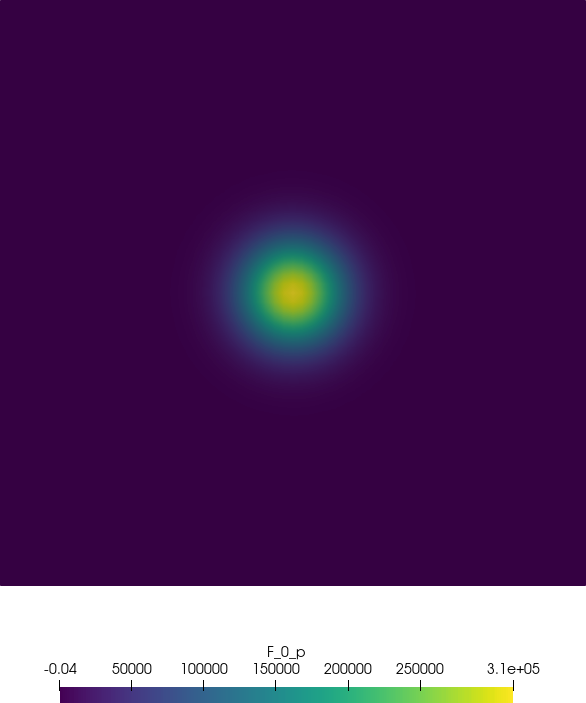
\includegraphics[width=0.4\textwidth]{img/Acoustics_F_0_p.png} \hfill%
	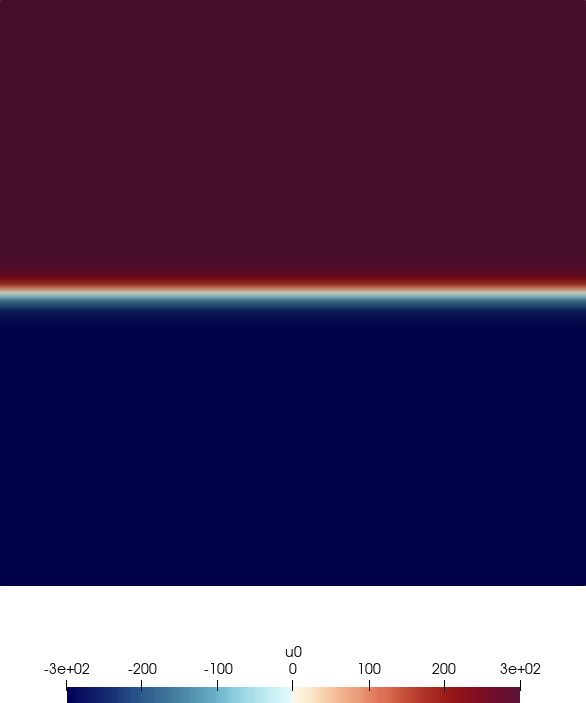
\includegraphics[width=0.4\textwidth]{img/Acoustics_u0.png}
    \vspace{5mm}\\%
	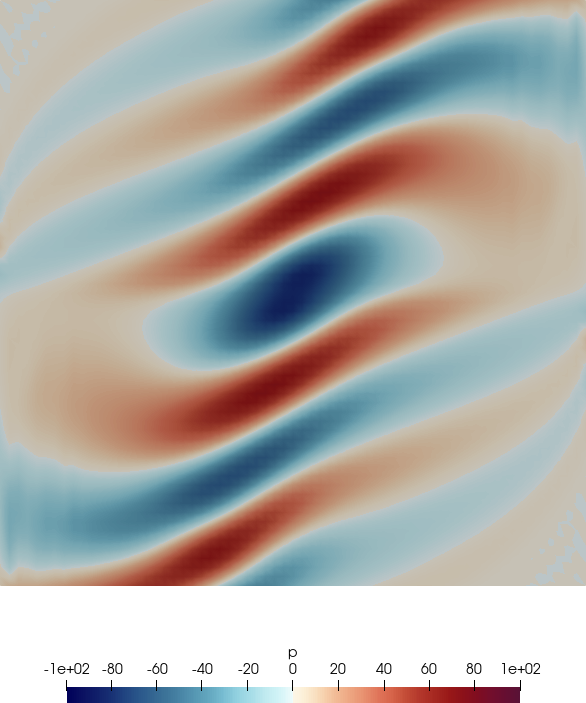
\includegraphics[width=0.4\textwidth]{img/Acoustics_p.png} \hfill%
	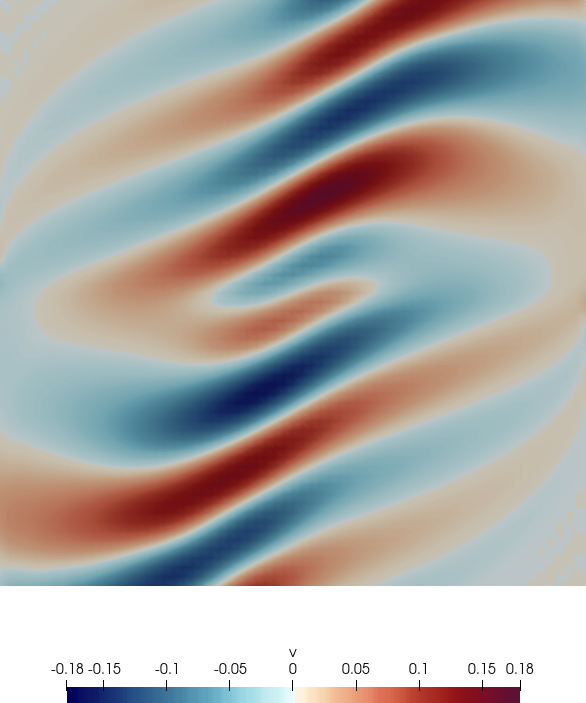
\includegraphics[width=0.4\textwidth]{img/Acoustics_v.png}
	\caption{Acoustic source term, base flow velocity, acoustic pressure and acoustic velocity perturbations.}
	\label{f:acousticsolver:results}
\end{figure}

